\documentclass[a4paper,12pt]{article} %style de document
\usepackage[utf8]{inputenc} %encodage des caractères
\usepackage[french]{babel} %paquet de langue français
\usepackage[T1]{fontenc} %encodage de la police
\usepackage[top=2cm,bottom=2cm,left=2cm,right=2cm]{geometry} %marges
\usepackage{graphicx} %affichage des images
\usepackage{amssymb}
\usepackage{url}
\usepackage{verbatim}
\usepackage{amsmath}
\usepackage{color}
\usepackage{tikz}
\usepackage{hyperref}
\usepackage{listings}
\hypersetup{
	hidelinks,
    colorlinks,
    citecolor=black,
    filecolor=black,
    linkcolor=black,
    urlcolor=black
}

\begin{document} %début du document

%----------------------------------
%page de garde
%----------------------------------

\begin{titlepage}

\vspace{7cm}

\begin{center}

\begin{Huge}
Rapport Android\\
\end{Huge}
\vspace{2cm}
\begin{large}
Chagneux Dimitri 21606807\\
Mori Baptiste 21602052\\
Leblond Valentin 21609038\\
\vspace{1cm}
Lien du projet:\\
\url{https://github.com/BaptisteMori/Application_vente_immobiliere_Android}\\
\vspace{1cm}
L3-Informatique
\end{large}

\end{center}
\end{titlepage}


%------------------------------
%sommaire
%------------------------------

\newpage

\tableofcontents

\newpage

%------------------------------
%contenu
%------------------------------


\section{Présentation du sujet}

L'objectif de ce devoir était de réaliser une application de vente de biens immobiliers.

\section{Fonctionnalités implémentées}

\subsection{Liste de biens}
Du côté de la récupération des annonces en ligne, nous avons commencé par créer une requête pour aller chercher le fichier en ligne.
A partir de la le résultat obtenu est un fichier au format json , ce qui implique l'utilisation de la librairie Moshi pour parser ce fichier. \\
Pour cela nous avons créé dans un premier temps un parseur pour traiter le cas où il n'y a qu'une seul propriété puis un second parseur pour le cas où il y a plusieurs annonces.\\
Nous avons été obligés de gérer ces deux cas car dans le cas où il y a plusieurs annonces celles-ci sont dans une liste contrairement au cas où il n'y en a qu'une seul.\\
Une fois la liste des propriétés récupérées, nous l'affichons dans la vue principale de l'application, dans un LinearLayout.

\subsection{Base de donnée local}
Nous avons séparés la base de donnée en trois tables une pour les propriétés, une pour les vendeurs et une pour les remarques qui peuvent être faite sur une propriété quand celle-ci est sauvegardée en local. La table remarque possède deux colonnes une avec l'identifiant de la propriété sur laquelle elle repose et la deuxième sur le texte que contient la remarque.

\begin{center}
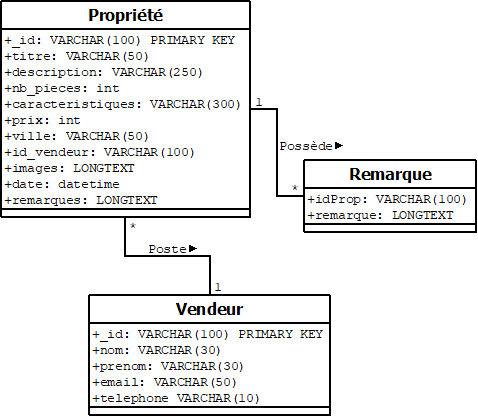
\includegraphics[scale=0.5]{images/bdd.png}
\end{center}

Nous avons essayé d'utiliser Room pour construire la partie base de données seulement nous avons rencontrés des problèmes dans la balise du getAll, nous avions une erreur sur le nom de la table qui était qu'il ne la trouvait pas (sachant que nous avions mis les balises @ColumnInfo avant chaque attribut de la classe Propriete).
\begin{lstlisting}
@Query("SELECT * FROM Propriete")
List<Propriete> getAll();
\end{lstlisting}

Ne trouvant pas comment résoudre le problème, nous avons finis par faire la base de donnée à la main, comme vu en TP, avec trois classes une classe VentesImmobilieresContract qui permet de mettre les noms des tables et de leurs colonnes ainsi que le nom de la base de donnée, la seconde classe VentesImmobilieresDBOpener permet de pouvoir créer et supprimer les tables selon si la base de donnée est crée, supprimée ou mise à jour. La dernière classe VentesImmobilieresDB permet de faire les requêtes sur la base de donnée.  

\subsection{Visualisation d'un bien}
La visualisation d'une propriété se fait sur une activité appelée ActivityAnnonce.
On y affiche le titre, une galerie d'images, le prix et la localisation, une description et des informations sur le vendeur. On ajoute en plus, si la propriété est sauvegardée dans la base de donnée locale, une liste de remarques.

\subsection{Menus}
Notre application dispose de deux menus: le premier est celui qui se trouve sur la première activité, lorsqu'on démarre l'application. Il permet d'accéder à la liste des propriétés sauvegardées en local. Le second est celui de l'activité qui affiche une annonce. On y trouve:\\
    -un bouton pour aller sur la liste de toutes les annonces (menu);\\
    -un bouton pour prendre une photo;\\
    -un bouton permettant d'enregistrer l'annonce en local, qui affiche un message dans une snackbar si l'annonce est déjà présente dans la base de donnée;\\
    -un bouton pour supprimer l'annonce de la base de donnée locale, qui affiche également un message dans une snackbar si l'annonce n'est pas dans la base;\\
    -un bouton listant les annonces sauvegardées en local (de la même manière que dans le premier menu);\\
    -un bouton pour ajouter une remarque si l'annonce se trouve en local. Dans le cas contraire on affiche un message dans une snackbar.

\subsection{Remarques et photos}
En ce qui concerne les remarques, il est possible d'en ajouter si la propriété se trouve sur la base de donnée en local. Si c'est le cas, en cliquant sur le bouton du menu d'une annonce on arrive sur une nouvelle vue contenant un champ de texte, un bouton retour et un bouton valider.
Au clique sur le bouton valider, la remarque est ajoutée en base de donnée et s'affiche sur la vue de l'annonce concernée. Elle est supprimée si l'annonce est supprimée de la base de données locale.
\vspace{1cm}

Pour les photos, l'appui sur l'icône de l'appareil photo ouvre l'application caméra par défaut, seulement si l'annonce est sauvegardée en locale.\\
Une fois la photo prise, on l'enregistre dans les fichiers de l'application avec un nom du type JPEG-yyyyMMdd-HHmmss.jpg". On ajoute ensuite le chemin de l'image dans la liste des images de l'application.

\section{Gestion du projet}

\subsection{Organisation}
Commun:\\
-Débuts de l'application (vue d'une annonce, lister des annonces codées en dur)
\vspace{0.5cm}

Baptiste:\\
-Moshi\\
-Aide sur les autres aspects
\vspace{0.5cm}

Valentin:\\
-Base de données
-Remarques (base de données)\\
-Aide sur les autres aspects\\
-Aspects graphiques (liste des annonces)
\vspace{0.5cm}

Dimitri:\\
-Liste des annonces, à partir du Moshi, dans une vue\\
-Remarques\\
-Prise de photos

\subsection{Difficultés}
L'une des grosses difficulté à été le parseur avec Moshi, la façon dont il fonctionne est assez flou. De plus l'adapter avec le fichier json fournis était un défi, du fait que le fichier avait une structure particulière.

\end{document}
